\documentclass{standalone}
\usepackage{tikz}

\begin{document}
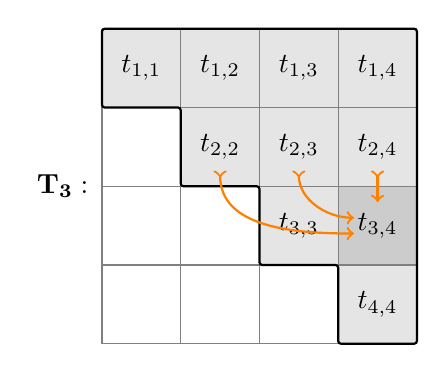
\begin{tikzpicture}[scale=1,every node/.style={minimum size=0.5cm}]

  \begin{scope}
    \fill[white,fill opacity=0.8] (0.0,0.0) rectangle (4.0,4.0);

    \fill[gray!20] (0,4) -- (0,3) -- (1,3) -- (1,2) -- (2,2) -- (2,1) -- (3,1) -- (3,0) -- (4,0) -- (4,4) -- cycle;

    \fill[gray!40] (3,2) -- (4,2) -- (4,1) -- (3,1) -- cycle;

    \draw[step=10mm, thin, gray] (0.0,0.0) grid (4.0,4.0);
    \draw[black, thick, rounded corners=1] (0,4) -- (0,3) -- (1,3) -- (1,2) -- (2,2) -- (2,1) -- (3,1) -- (3,0) -- (4,0) -- (4,4) -- cycle;

    \node at (0.5, 3.5) [black] {$t_{1,1}$};
    \node at (1.5, 3.5) [black] {$t_{1,2}$};
    \node at (2.5, 3.5) [black] {$t_{1,3}$};
    \node at (3.5, 3.5) [black] {$t_{1,4}$};
    \node at (1.5, 2.5) [black] {$t_{2,2}$};
    \node at (2.5, 2.5) [black] {$t_{2,3}$};
    \node at (3.5, 2.5) [black] {$t_{2,4}$};
    \node at (2.5, 1.5) [black] {$t_{3,3}$};
    \node at (3.5, 1.5) [black] {$t_{3,4}$};
    \node at (3.5, 0.5) [black] {$t_{4,4}$};

    \draw[>->, orange, thick] (2.5, 2.2) to[out=270,in=180] (3.2, 1.6);
    \draw[>->, orange, thick] (3.5, 2.2) to[out=270,in=90] (3.5, 1.8);
    \draw[>->, orange, thick] (1.5, 2.2) to[out=270,in=180] (3.2, 1.4);
  \end{scope}

  \node at (-0.5, 2) [black] {$\mathbf{T_3}:$};
\end{tikzpicture}
\end{document}